\chapter{Exploring $N = 3$ with a Hermite Algorithm}

Having seen the dramatic improvement that came from switching from the
forward Euler algorithm to the leapfrog, the obvious next step was to
go to yet higher order algorithms.  A quick look in a few books of
numerical methods showed our friends that there was a bewildering
choice of third- and fourth-order methods to choose from.  Alice then
mentioned that her thesis advisor had pointed her to an elegant and
natural generalization of the leapfrog algorithm, by the name of the
Hermite scheme.

\section{A Surprisingly Simple Hermite Scheme}

The most symmetric Hermite version, and the one closest resembling the
leapfrog is this one:

\def\half{{\textstyle\frac{1}{2}}}
\def\quarter{{\textstyle\frac{1}{4}}}
\def\one#1{{\textstyle\frac{1}{#1}}}
\def\three#1{{\textstyle\frac{3}{#1}}}
\def\seven#1{{\textstyle\frac{7}{#1}}}

\begin{eqnarray}
\br_{i+1} & = & \br_i + \half(\bv_i + \bv_{i+1}) dt +
                \one{12}(\ba_i - \ba_{i+1})(dt)^2
                \label{hermite-step1} \\
\bv_{i+1} & = & \bv_i + \half(\ba_i + \ba_{i+1}) dt +
                \one{12}(\bj_i - \bj_{i+1})(dt)^2
                \label{hermite-step2}
\end{eqnarray}

Here $\bj = d\ba/dt$ is the {\it jerk}, the time derivative of the
acceleration, and therefore the third time derivative of position:

\begin{equation}
\bj = \frac{d^3}{dt^3} \br
\end{equation}

The term `jerk' has crept into the literature relatively recently,
probably originally as a pun.  If a car or train changes acceleration
relatively quickly you experience not a smoothly accelerating or
decelerating motion, but instead a rather `jerky' one.

The jerk can be computed through straightforward differentiation of
Newton's gravitational equations, Eq. \ref{newton}:

\begin{equation}
\bj_i =  G \sum_{j=1 \atop j \neq i}^N \,M_j \left[
\frac{\bv_{ji}}{r_{ji}^3} - 3 \frac{(\br_{ji}\cdot\bv_{ji})\br_{ji}}{r_{ji}^5}
\right]\label{newton-jerk}
\end{equation}

\noindent
where $\bv_{ji} = \bv_j - \bv_i$.

As an aside, note that the jerk has one very convenient property.
Although the expression above looks quite a bit more complicated than
Newton's original equations, they can still be evaluated through one
pass over the whole $N$-body system.  This is no longer true for
higher derivatives.  For example, we can obtain the fourth derivative
of the position of particle $i$ (the {\it snap}, see next section) by
differentiating Eq. \ref{newton-jerk}:

\begin{eqnarray}
\frac{d^4}{dt^4}\br_i = G \sum_{j=1 \atop j \neq i}^N \,M_j \Bigg[ &\,&
\!\!\!\!\!\!\!\!\!\! \frac{\ba_{ji}}{r_{ji}^3}
-6 \frac{(\br_{ji}\cdot\bv_{ji})}{r_{ji}^5}\bv_{ji} \nonumber \\
 &\,& \!\!\!\!\!\!\!\! + \left\{ -3\frac{v_{ji}^2}{r_{ji}^5}
-3 \frac{(\br_{ji}\cdot\ba_{ji})}{r_{ji}^5}
+15 \frac{(\br_{ji}\cdot\bv_{ji})^2}{r_{ji}^7} \right\} \br_{ji} \,\,\Bigg]
\label{newton-snap}
\end{eqnarray}

\noindent
where $\ba_{ji} = \ba_j - \ba_i$, and this is the expression that
thickens the plot.  Unlike the $\br_{ji}$ and $\bv_{ji}$ expressions,
that are given by the initial conditions, $\ba_{ji}$ has to be
calculated from the positions and velocities.  However, this
calculation does not only involve the pairwise attraction of particle
$j$ on particle $i$, but in fact all pairwise attractions of all
particles on each other!  This follows immediately when we write out
what the shorthand implies:

\begin{equation}
\ba_{ji} = \ba_j - \ba_i = G \sum_{k=1 \atop k \neq j}^N
\frac{M_k}{r_{kj}^3} \,\br_{kj} -  G \sum_{k=1 \atop k \neq i}^N
\frac{M_k}{r_{ki}^3} \,\br_{ki}
\end{equation}

\noindent
When we substitute this back into Eq. \ref{newton-snap}, we see that
we have to do a double pass over the $N$-body system, summing over
both indices $k$ and $j$ in order to compute a single fourth derivative
for the position of particle $i$.  

\section{Comparison with the Leapfrog}

When we look at Eqs. \ref{hermite-step1}, \ref{hermite-step2}, we see
some familiar features.  Neglecting the higher-order term for the
moment, we recognize the leapfrog: the new position is effectively
determined by the mid-point velocity $v_{i+1/2}$, here approximated as
the average between the two adjacent values $v_{i}$ and $v_{i+1}$.
Similarly, the new velocity is effectively determined by the mid-point
acceleration.

In fact, the analogy can be made more precise.  Recalling the leapfrog,
as written centered on integer times, Eqs. \ref{leapfrog-step1},
\ref{leapfrog-step2}:

\begin{eqnarray}
\br_{i+1} & = & \br_i + \bv_{i} dt + \ba_{i} (dt)^2/2 \label{leapfrog-step1a}\\
\bv_{i+1} & = & \bv_i + (\ba_i + \ba_{i+1})dt / 2 \label{leapfrog-step2a}
\end{eqnarray}

\noindent
we can transform these back into a pseudo-leap form, without using
half-integer times explicitly, by rewriting the first equation as:

\begin{eqnarray}
\br_{i+1} & = & \br_i + \half(\bv_{i} + \bv_{i+1}) dt
                      + \half(\bv_{i} - \bv_{i+1}) dt
                      + \half\ba_{i} (dt)^2 \nonumber \\
	  & = & \br_i + \half(\bv_{i} + \bv_{i+1}) dt
                      + \quarter(-\ba_i-\ba_{i+1})(dt)^2
                      + \half\ba_{i}(dt)^2 \nonumber \\
	  & = & \br_i + \half(\bv_{i} + \bv_{i+1}) dt
                      + \quarter(\ba_i-\ba_{i+1})(dt)^2 \nonumber \\
	  & = & \br_i + \half(\bv_{i} + \bv_{i+1}) dt - \quarter\bj_i (dt)^3
                                                      \label{leapfrog-trick}
\end{eqnarray}

In the second line, we have simply rearranged terms.  In the third
line, we have used \ref{leapfrog-step2a}, and in the fourth line we
have used the definition of $\bj$, while neglecting higher order terms
in $dt$.

The next step is to remember that the leapfrog is a second-order scheme.
The errors per step are $\propto(dt^3)$, and therefore it does not
matter whether or not we include the last term $-\bj_i (dt)^3/4$ into
our leapfrog version: this term is lost in the noise, and is not going
to improve the accuracy on second-level order.  Therefore, we may
equally well leave it out.  Doing so transforms Eqs. \ref{leapfrog-step1a},
\ref{leapfrog-step2a} into:

\begin{eqnarray}
\br_{i+1} & = & \br_i + \half(\bv_i + \bv_{i+1})dt \label{leapfrog-step1b} \\
\bv_{i+1} & = & \bv_i + \half(\ba_i + \ba_{i+1})dt \label{leapfrog-step2b}
\end{eqnarray}

Here we see explicitly that our good old leapfrog is equivalent, up to
its second-order accuracy, with the leading terms $\propto (dt)$ of
the Hermite algorithm, Eqs. \ref{hermite-step1}, \ref{hermite-step2}.
It is a curiosity of the leapfrog that at first sight it resembles a
first-order scheme, since the second-order terms are hidden in the
`leapy' way of using average quantities.  Yet, as we have seen, the
leapfrog is fully second-order.

In a very similar way, the Hermite scheme is fourth-order, even though
it resembles a second-order scheme.  For details we refer to the
literature, but it is interesting to see in a heuristic way why this
is so.

\section{Snap, Crackle, and Pop}

First a word about terminology.  We will need to introduce a few extra
derivatives of the position.  It would be fun to give them names with
a reasonable `feel' to them, just like with jerk.  What type of motion
feels even more restless than jerking motion?  A sudden snap comes to
mind.  A what changes its state more sudden than a snap --- how about
a crackle?  And for those familiar with American rice crispies culture,
a pop cannot be far away, and indeed, if something pops it really
changes high derivatives of positions in a substantial way!  We are
not making these names up: we have seen them used a few times before,
although the precise source is likely to be lost in (recent) history.
So here they are:

\begin{equation}
\bs = \frac{d^4}{dt^4} \br \qquad ; \qquad
\bc = \frac{d^5}{dt^5} \br \qquad ; \qquad
\bp = \frac{d^6}{dt^6} \br
\end{equation}

\noindent
{\it snap}, {\it crackle}, and {\it pop}, respectively.

We are now in a position to write the Taylor series for the four
quantities that appear in Eqs. \ref{hermite-step1}, \ref{hermite-step2},
up to crackle:

\begin{eqnarray}
\br_{i+1} & = & \br_i + \bv_i dt + \half\ba_{i}(dt)^2 + \one{6}\bj_{i}(dt)^3
                      + \one{24}\bs_{i}(dt)^4 + \one{120}\bc_{i}(dt)^5
                                                           \label{taylor-r} \\
\bv_{i+1} & = & \bv_i + \ba_i dt + \half\bj_{i}(dt)^2 + \one{6}\bs_{i}(dt)^3
                      + \one{24}\bc_{i}(dt)^4              \label{taylor-v} \\
\ba_{i+1} & = & \ba_i + \bj_i dt + \half\bs_{i}(dt)^2 + \one{6}\bc_{i}(dt)^3
                                                           \label{taylor-a} \\
\bj_{i+1} & = & \bj_i + \bs_i dt + \half\bc_{i}(dt)^2      \label{taylor-j}
\end{eqnarray}

\noindent
We can now eliminate snap and crackle at time $t_i$, expressing them
in terms of the acceleration and jerk at times $t_i$ and $t_{i+1}$,
using Eqs. \ref{taylor-a}, \ref{taylor-j}.  We find:

\begin{eqnarray}
\bs_i &=& 6(\ba_{i+1} -\ba_{i})(dt)^{-2} -2(\bj_{i+1} +2\bj_{i})(dt)^{-1} \\
\bc_i &=& -12(\ba_{i+1} -\ba_{i})(dt)^{-3} +6(\bj_{i+1} +\bj_{i})(dt)^{-2}
\end{eqnarray}

\noindent
Substituting both expressions in Eq. \ref{taylor-v} we directly find:

\begin{equation}
\bv_{i+1} = \bv_i + \half(\ba_i + \ba_{i+1}) dt +
                \one{12}(\bj_i - \bj_{i+1})(dt)^2 \label{hermite-step2a}
\end{equation}

\noindent
Indeed, we have recovered Eq. \ref{hermite-step2}, and thereby
explained the mysterious factor $\one{12}$ in the last term.

Let us complete our mission, by making the same derivation for 
the position vector, Eq. \ref{hermite-step1}, in the Hermite scheme.
Using again the snap and crackle expressions derived above, we find:

\begin{equation}
\br_{i+1} = \br_i + \bv_i dt + (\seven{20}\ba_i + \three{20}\ba_{i+1})(dt)^2
            + (\one{20}\bj_i - \one{30}\bj_{i+1})(dt)^3
\end{equation}

\noindent
Using the same trick we employed in Eq. \ref{leapfrog-trick} to factor
out the velocity terms, and using Eq. \ref{hermite-step2a}, we can
rewrite the above expression as:

\begin{equation}
\br_{i+1} = \br_i + \half(\bv_i + \bv_{i+1}) dt
            + \one{10}(\ba_i - \ba_{i+1})(dt)^2
            + \one{120}(\bj_i + \bj_{i+1})(dt)^3
\end{equation}

\noindent
While this result still looks quite different from Eq. \ref{hermite-step1},
we claim that it is identical up to fourth-order in $dt$, which is all we
need.  Our final step thus parallels the discussion following
Eq. \ref{leapfrog-trick} for the leapfrog, where we had to show how
terms up to second-order were identical.

First we rewrite the above equation in terms of quantities defined at $t=i$:

\begin{eqnarray}
\br_{i+1} = \br_i + \half(\bv_i + \bv_{i+1}) dt 
             & + & \one{10}\ba_i(dt)^2 - \one{10}(\ba_i + \bj_i dt +
              \half\bs_i (dt)^2)(dt)^2                           \nonumber \\
          & + & \one{120}\bj_i(dt)^3 + \one{120}(\bj_i + \bs_i dt)(dt)^3
                                                                 \nonumber \\
          = \br_i + \half(\bv_i + \bv_{i+1}) dt 
          & - & \one{12}\bj_i (dt)^3 - \one{24} \bs_i (dt)^4
\end{eqnarray}

\noindent
Here we have left out terms containing $\bc_i$, since they would be
proportional to at least $(dt^5)$ and only contribute to the error noise.
We can similarly write out the last term of Eq. \ref{hermite-step1}:

\begin{eqnarray}
\one{12}(\ba_i - \ba_{i+1})(dt)^2  & = & 
              \one{12}\left(\ba_i(dt)^2 - \one{12}(\ba_i + \bj_i dt +
              \half\bs_i (dt)^2)\right)(dt)^2                     \nonumber \\
             & = & - \one{12}\bj_i (dt)^3 - \one{24} \bs_i (dt)^4
\end{eqnarray}

\noindent
This proves the desired result:

\begin{equation}
\br_{i+1} = \br_i + \half(\bv_i + \bv_{i+1}) dt +
                \one{12}(\ba_i - \ba_{i+1})(dt)^2
\end{equation}

\section{Implementing Hermite}

Let us return to Alice, Bob, and Carol, who are about to implement the
Hermite scheme.  Since Bob was most eager to test out this new
algorithm, he got his turn behind the computer.

\abc

\bob
Let's give this new Hermite scheme a stress test.  I'll take {\st
leapfrog2a.C}, the one with the off-set in initial velocity of
$10^{-4}$, call it {\st hermite1a.C} for now, and simply substitute
the leapfrog equations \ref{leapfrog-step1}, \ref{leapfrog-step2} by
the Hermite equations \ref{hermite-step1}, \ref{hermite-step2}.

\carol
Why not call the code {\st hermite1.C}?

\bob
Even though the update seems almost trivial, I don't have the audacity
to believe we'll get everything right the first time around.  When it
all works, we will rename the code to {\st hermite1.C}.  So here is
the new version:

\cba

\code{hermite1a.C}{chap6/hermite1a.C}

\abc

\alice
Ah, I see now that you were wise giving the code an preliminary name.
Notice where you have added the jerk calculation.  You replaced

\begin{small}
\begin{verbatim}
            for (int k = 0; k < 3; k++){
                a[i][k] += m * rji[k] / r3;
                a[j][k] -= m * rji[k] / r3;
            }
\end{verbatim}
\end{small}

\noindent
by:

\begin{small}
\begin{verbatim}
            for (int k = 0; k < 3; k++){
                a[i][k] += m * rji[k] / r3;
                a[j][k] -= m * rji[k] / r3;
                jk[i][k] += m * (vji[k] - 3 * rv * rji[k]) / r3;
                jk[j][k] -= m * (vji[k] - 3 * rv * rji[k]) / r3;
            }
\end{verbatim}
\end{small}

\noindent
in addition to some extra changes, such as introducing and calculating
the variable {\st vji[]} for the relative velocities for particles $i$
and $j$.  All of this is fine, as far as I can see.  The statements are
correctly written and reflect the Hermite, but there is one problem.
In the last two lines above you use the relative velocities $vij[]$,
but at this point in the program they have not been assigned yet.

\bob
Ah, you are right.  That happens just a few lines below, with this
`clever' trick of using the magnitude of the centrifugal acceleration
to determine the magnitude of the velocities.  Thanks!  Okay, so I'll
make another version, {\st hermite1b.C}, which has two initial loops,
one for the accelerations, followed by the assignment of velocities,
and then followed by the second loop which computes the jerks.

\carol
Maybe we can just run the program using our friend {\st /dev/null} to
see how the energy behaves, before start making pictures.  I'm really
curious to see whether we have now reached fourth-order accuracy.

\bob
Easy to test:

\cba

\begin{small}
\begin{verbatim}
|gravity> g++ -o hermite1b hermite1b.C
|gravity> hermite1b > /dev/null
Please provide a value for the time step
0.01
and for the duration of the run
100
Initial total energy E_in = -0.866025
Final total energy E_out = -0.975389
absolute energy error: E_out - E_in = -0.109364
relative energy error: (E_out - E_in) / E_in = 0.126282
|gravity> !!
hermite1b > /dev/null
Please provide a value for the time step
0.001
and for the duration of the run
100
Initial total energy E_in = -0.866025
Final total energy E_out = -0.866586
absolute energy error: E_out - E_in = -0.000560173
relative energy error: (E_out - E_in) / E_in = 0.000646832
|gravity> !!
hermite1b > /dev/null
Please provide a value for the time step
0.0001
and for the duration of the run
100
Initial total energy E_in = -0.866025
Final total energy E_out = -0.866026
absolute energy error: E_out - E_in = -5.52839e-07
relative energy error: (E_out - E_in) / E_in = 6.38364e-07
|gravity> !!
hermite1b > /dev/null
Please provide a value for the time step
0.00001
and for the duration of the run
100
Initial total energy E_in = -0.866025
Final total energy E_out = -0.866025
absolute energy error: E_out - E_in = -5.53711e-10
relative energy error: (E_out - E_in) / E_in = 6.39371e-10
|gravity> 
\end{verbatim}
\end{small}

\abc

\carol
What is this?  We seem to have constructed a third-order algorithm!

\alice
Hmmm.  It seems that way.  Each refinement of a factor ten in step
size gives a reduction of the error of a factor 1000.  But this was
not supposed to happen

\bob
This is strange indeed.  Look, at the end, there they are, the real
Hermite expressions, what can be wrong with such simple statements??

\begin{small}
\begin{verbatim}
        for (int i = 0; i < n; i++){
            for (int k = 0; k < 3; k++){
                r[i][k] = old_r[i][k] + (old_v[i][k] + v[i][k])*dt/2
                                      + (old_a[i][k] - a[i][k])*dt*dt/12;
                v[i][k] = old_v[i][k] + (old_a[i][k] + a[i][k])*dt/2
                                      + (old_j[i][k] - jk[i][k])*dt*dt/12;
            }
        }
\end{verbatim}
\end{small}

\carol
Yes, they are just what we derived before, as Eqs. \ref{hermite-step1},
\ref{hermite-step2}.

\alice
Could we have made a similar mistake as we did just before, when the
expressions were absolutely correct, but the order of execution was wrong?

\bob
Well \dots hmmm \dots aha, of course, you are right!  Look, that is
exactly the problem.  In the first line, where the position is updated,
we indicate that we are using both the old velocity values and the new
velocity values.  However, the new ones have not been computed yet ---
that happens only on the next line!  And the solution is obvious:
fortunately, the second line updating the velocity does not have this
problem, since it uses only accelerations and jerks, all of which have
already been computed, both for the old and the new values.  So we can
simply swap the lines, and this should now work:

\begin{small}
\begin{verbatim}
        for (int i = 0; i < n; i++){
            for (int k = 0; k < 3; k++){
                v[i][k] = old_v[i][k] + (old_a[i][k] + a[i][k])*dt/2
                                      + (old_j[i][k] - jk[i][k])*dt*dt/12;
                r[i][k] = old_r[i][k] + (old_v[i][k] + v[i][k])*dt/2
                                      + (old_a[i][k] - a[i][k])*dt*dt/12;
            }
        }
\end{verbatim}
\end{small}

\section{Testing the Hermite: Three Stars on a Circle}

\bob
Now I'm ready to be brave and call the code {\st hermite1.C}.  Rather
than listing the whole output, let me use the {\st diff} program,
which only lists those lines that are different.

\cba

\begin{small}
\begin{verbatim}
|gravity> diff hermite1a.C hermite1.C
2c2
< // hermite1a.C
---
> // hermite1.C
30c30
<             a[i][k] = jk[i][k] = 0.0;
---
>             a[i][k] = 0.0;
33,34c33,34
<             double rji[3], vji[3];
<             for (int k = 0; k < 3; k++){
---
>             double rji[3];
>             for (int k = 0; k < 3; k++)
36,37d35
<                 vji[k] = v[j][k] - v[i][k];
<             }
42,45d39
<             double rv = 0;
<             for (int k = 0; k < 3; k++)
<                 rv += rji[k] * vji[k];
<             rv /= r2;
49,50d42
<                 jk[i][k] += m * (vji[k] - 3 * rv * rji[k]) / r3;
<                 jk[j][k] -= m * (vji[k] - 3 * rv * rji[k]) / r3;
64a57,81
>     for (int i = 0; i < n; i++)
>         for (int k = 0; k < 3; k++)
>             jk[i][k] = 0.0;
>     for (int i = 0; i < n; i++){
>         for (int j = i+1; j < n; j++){
>             double rji[3], vji[3];
>             for (int k = 0; k < 3; k++){
>                 rji[k] = r[j][k] - r[i][k];
>                 vji[k] = v[j][k] - v[i][k];
>             }
>             double r2 = 0;
>             for (int k = 0; k < 3; k++)
>                 r2 += rji[k] * rji[k];
>             double r3 = r2 * sqrt(r2);
>             double rv = 0;
>             for (int k = 0; k < 3; k++)
>                 rv += rji[k] * vji[k];
>             rv /= r2;
>             for (int k = 0; k < 3; k++){
>                 jk[i][k] += m * (vji[k] - 3 * rv * rji[k]) / r3;
>                 jk[j][k] -= m * (vji[k] - 3 * rv * rji[k]) / r3;
>             }
>         }
>     }
> 
127,128d143
<                 r[i][k] = old_r[i][k] + (old_v[i][k] + v[i][k])*dt/2
<                                       + (old_a[i][k] - a[i][k])*dt*dt/12;
130a146,147
>                 r[i][k] = old_r[i][k] + (old_v[i][k] + v[i][k])*dt/2
>                                       + (old_a[i][k] - a[i][k])*dt*dt/12;
|gravity>
\end{verbatim}
\end{small}

\abc

\carol
Yes, that is much clearer than listing the whole source code again.
I can see how the main difference has been the move of the jerk
calculation from the earlier part, where it was entangled with the
acceleration calculation, to a separate block listed nearly at the
end.  At the very end, of course, there is the indication that we have
swapped the order of the calculations of the positions and the velocities.
The {\st diff} program arbitrarily took the velocity calculation as a
identical standard in each file, with respect to which the shift in
order of the position calculation was noted.

\alice
Soon we should start to clean up our codes, splitting them in
functions at least, and probably also in different files.  That way we
don't have to rely on {\st diff} to read our own programs, since we
can then take natural chunks at a time, in the form of functions.  But
first let's see what will happen to our figure 8 orbits.

\bob
Here are the results.  Hmm, not a very good energy conservation, if
you ask me.

\cba

\begin{small}
\begin{verbatim}
|gravity> g++ -o hermite1 hermite1.C
|gravity> hermite1 > hermite1_0.01_100.out
Please provide a value for the time step
0.01
and for the duration of the run
100
Initial total energy E_in = -0.866025
Final total energy E_out = -1.08608
absolute energy error: E_out - E_in = -0.220054
relative energy error: (E_out - E_in) / E_in = 0.254096
|gravity>
\end{verbatim}
\end{small}

\abc

\carol
Indeed.  The leapfrog did far better at this stage.  We got a relative
energy error of less than $10^{-3}$, and here we are faced with a relative
energy error of a quarter!

\alice
That is not so strange, actually.  A higher-order algorithm computes
higher-order derivatives, and therefore can be extra sensitive to
close encounters or other situations in which changes happen quite
suddenly.  Let's look at the picture, and then move on, refining our
step size.

\cba

\begin{figure}[htb]
\centering
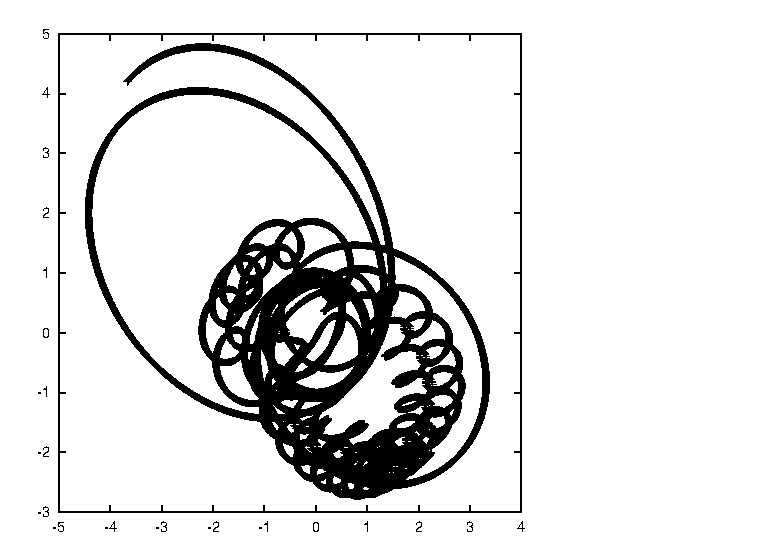
\includegraphics[width=2.5in]{chap6/hermite1_0.01_100.ps}
\caption[Three stars on a circle, Hermite, $dv_{init}=0.0001$, $dt = 0.01$,
$t_{end} = 100$]
{The first Hermite attempt to integrate the orbits of three stars
starting off on a circle with an initial velocity perturbation of 
$dv_{init}=0.0001$, time step $dt = 0.01$ and a total duration of
$t_{end} = 100$}
\label{fig:hermite1-0.01-100}
\end{figure}

\begin{small}
\begin{verbatim}
|gravity> hermite1 > hermite1_0.001_100.out
Please provide a value for the time step
0.001
and for the duration of the run
100
Initial total energy E_in = -0.866025
Final total energy E_out = -0.866026
absolute energy error: E_out - E_in = -9.19142e-07
relative energy error: (E_out - E_in) / E_in = 1.06133e-06
|gravity>
\end{verbatim}
\end{small}

\begin{figure}[htb]
\centering
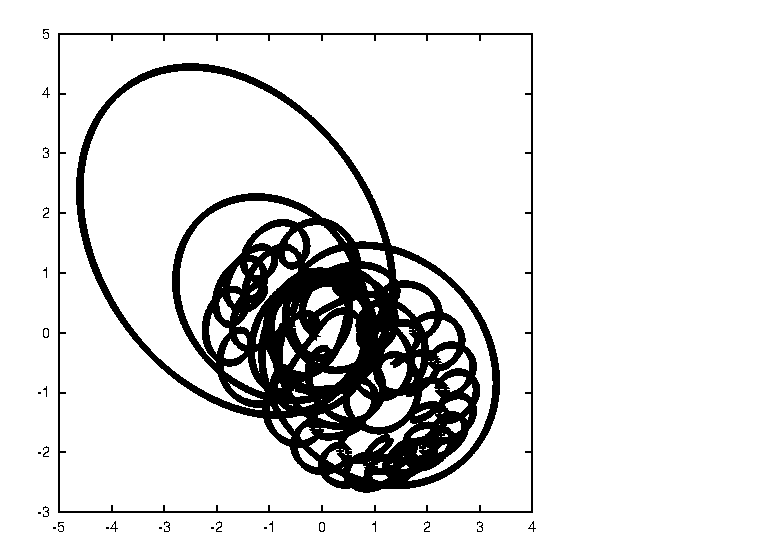
\includegraphics[width=2.5in]{chap6/hermite1_0.001_100.ps}
\caption[Three stars on a circle, Hermite, $dv_{init}=0.0001$, $dt = 0.001$,
$t_{end} = 100$]
{The second Hermite attempt to integrate the orbits of three stars
starting off on a circle with an initial velocity perturbation of 
$dv_{init}=0.0001$, time step $dt = 0.001$ and a total duration of
$t_{end} = 100$}
\label{fig:hermite1-0.001-100}
\end{figure}

\abc

\carol
Ah, much better!  Amazing.

\bob
An improvement of more than a factor 100,000 in accuracy!

\carol
And look at the picture.  I cannot see any difference between Fig. 
\ref{fig:hermite1-0.001-100} and the last picture in the series that
we did with the leapfrog, Fig. \ref{fig:leap2a-0.00001-100}!

\alice
Let's take another refinement step, to see whether we can determine
the asymptotic behavior of the error growth.  Clearly, our first
attempt was not reliable, so we need at least a third try.

\cba

\begin{small}
\begin{verbatim}
|gravity> hermite1 > hermite1_0.0001_100.out
Please provide a value for the time step
0.0001
and for the duration of the run
100
Initial total energy E_in = -0.866025
Final total energy E_out = -0.866025
absolute energy error: E_out - E_in = -8.49854e-12
relative energy error: (E_out - E_in) / E_in = 9.81326e-12
|gravity>
\end{verbatim}
\end{small}

\begin{figure}[htb]
\centering
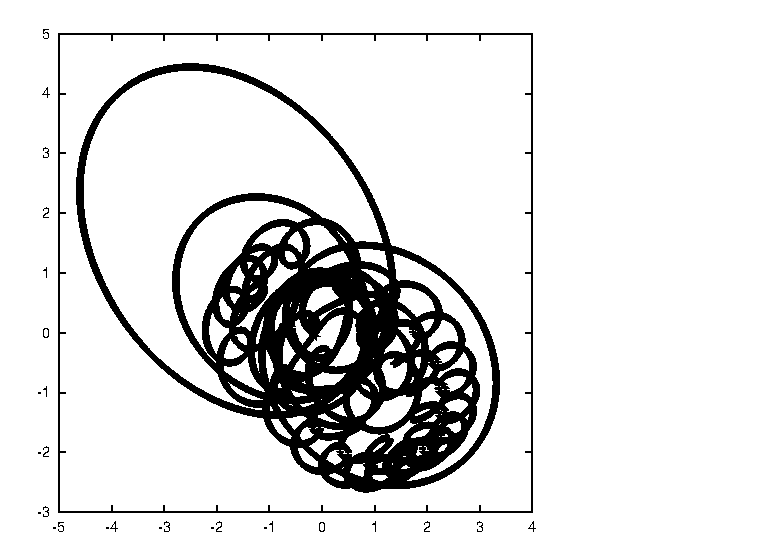
\includegraphics[width=2.5in]{chap6/hermite1_0.0001_100.ps}
\caption[Three stars on a circle, Hermite, $dv_{init}=0.0001$, $dt = 0.0001$,
$t_{end} = 100$]
{The third Hermite attempt to integrate the orbits of three stars
starting off on a circle with an initial velocity perturbation of 
$dv_{init}=0.0001$, time step $dt = 0.0001$ and a total duration of
$t_{end} = 100$}
\label{fig:hermite1-0.0001-100}
\end{figure}

\abc

\carol
Okay, Bob, you can call this code {\st hermite1.C}, it seems to do its job.

\bob
But it does its job too well.  Another five magnitudes of error improvement.
Now it behaves like a fifth order code.

\alice
This seems to happen sometimes.  A $k$th-order scheme is guaranteed
only to have errors that grow not faster than $k$th order.  However,
it is possible for them to grow less fast.  For example, it could be
that the particular orbits we are studying just happen to have some
properties that lead to cancellations in some of the orders.

\carol
Is there any reason to believe that we do not have a generic system here?

\alice
Don't forget that we are studying a rather unstable system, in which
it is quite likely that we will have at least one close encounter
between two or three particles.  So far, we have been sailing blindly,
hoping that the step size we give the integrator is small enough to
prevent near-collisions or other forms of strange behavior during
close encounters.  Soon we'll have to do better, though.  It is not
too hard to predict close encounters when they are about to happen,
and to adapt the integration step size automatically.  Only with such
safety precautions does it make sense to rigorously measure the
performance of the algorithm, whether it is the leapfrog or the
Hermite.  Without such precautions, even slight changes could show a
different behavior.  For example, cleaning up the code by initializing
the velocities directly, instead of using the centrifugal trick, is
likely to give slightly different initial conditions.  I would not
be surprised if such a change would give us yet another scaling of the
errors, if we repeat the above measurements.

\bob
Okay, I guess we are ready to do quite a bit of cleaning up in our code.
It is getting a bit too spaghetti-like for my taste already.  Let's do
that next time.  We can improve readability and functionality at the
same time, while we go along.

\carol
For now though, I feel that the Hermite should be our tool of choice.
It sure seems to converge must faster.  How about doing a timing test?

\bob
Good idea.  Let's do it with the figure-8 orbits though.  There at
least we do not have any close encounters, so Alice's warnings may
carry less urgency.

\cba

\section{The Hermite Soars: Three Bodies on a Figure Eight}

\abc

\bob
Here is the code.  Rather than doing another {\st diff}, since this is
a new problem I will list it in full.

\cba

\code{hermite2.C}{chap6/hermite2.C}

\abc

\bob
And here are the results.  Another fifth-order error behavior!

\cba

\begin{small}
\begin{verbatim}
|gravity> g++ -o hermite2 hermite2.C
|gravity> hermite2 > hermite2_0.01_100.out
Please provide a value for the time step
0.01
and for the duration of the run
100
Initial total energy E_in = -1.28705
Final total energy E_out = -1.28705
absolute energy error: E_out - E_in = -3.81996e-07
relative energy error: (E_out - E_in) / E_in = 2.96801e-07
|gravity>
\end{verbatim}
\end{small}

\begin{small}
\begin{verbatim}
|gravity> hermite2 > hermite2_0.001_100.out
Please provide a value for the time step
0.001
and for the duration of the run
100
Initial total energy E_in = -1.28705
Final total energy E_out = -1.28705
absolute energy error: E_out - E_in = -4.00457e-12
relative energy error: (E_out - E_in) / E_in = 3.11144e-12
|gravity>
\end{verbatim}
\end{small}

\begin{figure}[htb]
\centering
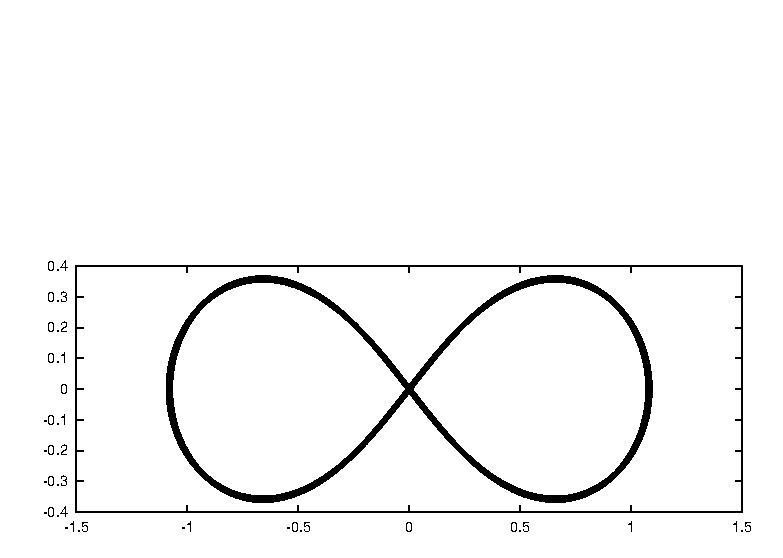
\includegraphics[width=4.5in]{chap6/hermite2_0.001_100.ps}
\caption[Three stars on a figure-8 orbit, Hermite, $dv_{init}=0.0001$,
$dt = 0.001$, $t_{end} = 100$]
{The second Hermite attempt to integrate the orbits of three stars
starting off on a figure-8 orbit with an initial velocity perturbation of 
$dv_{init}=0.0001$, time step $dt = 0.001$ and a total duration of
$t_{end} = 100$}
\label{fig:hermite2-0.001-100}
\end{figure}

\abc

\alice
Well, all I can say is that the regularity of the orbit probably gives
rise to cancellations.  This is a well-known phenomenon for the
leapfrog, for example, where sometimes the errors accumulate in the
phases more than the energies of the particles.  I suggest to come
back to this question by the time we try our hand at larger $N$-body
calculations starting from more random, less regular initial conditions.

\bob
Okay!  And here are the timings Carol asked for:

\cba

\begin{small}
\begin{verbatim}
|gravity> time leapfrog3a > /dev/null
Please provide a value for the time step
0.00001
and for the duration of the run
100
Initial total energy E_in = -1.287
Final total energy E_out = -1.287
absolute energy error: E_out - E_in = -1.24349e-11
relative energy error: (E_out - E_in) / E_in = 9.66196e-12
19.520u 0.100s 0:24.34 80.6%	0+0k 0+0io 168pf+0w
|gravity> time hermite2 > /dev/null
Please provide a value for the time step
0.001
and for the duration of the run
100
Initial total energy E_in = -1.28705
Final total energy E_out = -1.28705
absolute energy error: E_out - E_in = -4.00457e-12
relative energy error: (E_out - E_in) / E_in = 3.11144e-12
0.790u 0.010s 0:05.75 13.9%	0+0k 0+0io 169pf+0w
|gravity> 
\end{verbatim}
\end{small}

\abc

\carol
Not bad!  The Hermite is more accurate, even for time steps that are a
hundred times larger.  Of course, each time step is more complicated
than the leapfrog, so the time gain is less than a factor hundred, but
still considerable, about a factor twenty-five.

\alice
For this particular case, and also without optimization switched on.
Let's try compiling both programs with the $-O$ option of the g++
compiler, which should produce faster code.

\cba

\begin{small}
\begin{verbatim}
|gravity> g++ -O -o leapfrog3a leapfrog3a.C
|gravity> g++ -O -o hermite2 hermite2.C
|gravity> time leapfrog3a > /dev/null
Please provide a value for the time step
0.00001
and for the duration of the run
100
Initial total energy E_in = -1.287
Final total energy E_out = -1.287
absolute energy error: E_out - E_in = -1.20237e-11
relative energy error: (E_out - E_in) / E_in = 9.34243e-12
10.690u 0.060s 0:13.94 77.1%	0+0k 0+0io 165pf+0w
|gravity> time hermite2 > /dev/null
Please provide a value for the time step
0.001
and for the duration of the run
100
Initial total energy E_in = -1.28705
Final total energy E_out = -1.28705
absolute energy error: E_out - E_in = -4.06408e-12
relative energy error: (E_out - E_in) / E_in = 3.15768e-12
0.610u 0.020s 0:02.98 21.1%	0+0k 0+0io 165pf+0w
|gravity> 
\end{verbatim}
\end{small}

\abc

\carol
Aha!  Both programs ran faster, but the leapfrog more so.  Now Hermite
is ahead by `only' a factor 18 or so, instead of 25.

\alice
Still, for this particular case only.  And note that the energy errors
are now slightly different from before, without the optimizer switched
on.  Although the optimized code should in principle give the same
results as the non-optimized code if there would be no round-off
errors, in practice round-off does creep in and propagate into the
errors, especially when we are working at such high accuracies, where
we are relatively few bits away from machine precisions.  Fortunately, 
the effect does not seem to be too worrisome: we are talking about
relative differences in energy error of only a few percent.  But still
this is something we clearly have to be aware of.

\bob
Okay, enough warnings and footnotes!  Let's call it a night.  Next
time we get together we'll clean up the Hermite, and make it into a
general working tool.

\carol
Sounds good!  See you then.

\cba
